\ylDisplay{Valgusvihu laiendi} % Ülesande nimi
{Tundmatu autor} % Autor
{piirkonnavoor} % Voor
{2013} % Aasta
{P 5} % Ülesande nr.
{2} % Raskustase
{
% Teema: Valgusõpetus
\ifStatement
Laserist väljub paralleelne valgusvihk diameetriga $d = 2$ mm. Kasutades kumer- ja nõgusläätse muudetakse see paralleelseks valgusvihuks läbimõõduga $D = 6$ mm. Visandage optiline süsteem valgusvihu laiendamiseks ja arvutage nõgusläätse optiline tugevus, kui kasutatava kumerläätse fookuskaugus on $f = 15$ cm.
\fi
\ifHint
Nõgusläätse ja kumerläätse fookused peavad kattuma.
\fi
\ifSolution
\begin{center}
	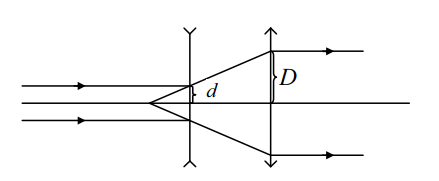
\includegraphics[width=0.5\linewidth]{2013-v2p-05-lah.PNG}
\end{center}
Nõguslääts ja kumerlääts paigutatakse üksteise taha ühele ja samale optilisele peateljele, nii et nende fookused kattuksid. \\
Seos $\frac{D}{f_{kumer}} = \frac{d}{f_{nõgus}}$ kolmnurkade sarnasusest. \\
Nõgusläätse fookuskauguse avaldamine: $f_{nõgus} = \frac{f_{kumer}d}{D} = 5$ cm. \\
Seosest $D = \frac{1}{f}$ nõgusläätse optiline tugevus $D = \frac{1}{-0,05 m} = -20$ dpt. \\
\fi
}
